\begin{enumerate}
  \item Một động cơ vận hành một băng chuyền nằm ngang với tốc độ không đổi, không phụ thuộc vào việc có vật nào đặt trên băng hay không. Một đĩa nặng khối lượng $m$ (ban đầu đứng yên) được đặt lên băng chuyền. Hệ số ma sát giữa đĩa và băng là $\mu$.
        \begin{figure}[H]
          \centering
          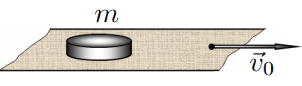
\includegraphics[width=0.35\textwidth]{Figures/Problems/Fig 1.1.png}
        \end{figure}
        \vspace{-0.5cm}
        Tính lượng nhiệt tỏa ra trong quá trình đĩa tăng tốc từ trạng thái tĩnh đến tốc độ của băng chuyền.
  \item Chất lỏng được bơm qua một ống nằm ngang với tốc độ không đổi. Một viên bi nhỏ khối lượng $m$ rơi vào trong ống. Lực ma sát nhớt do chất lỏng tác dụng lên viên bi có độ lớn tỉ lệ với vận tốc của viên bi: $F = -kv_{\text{rel}}$ trong đó $v_{\text{rel}}$ là vận tốc tương đối của viên bi so với chất lỏng. Bỏ qua lực cản từ thành ống.
        \begin{figure}[H]
          \centering
          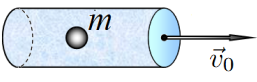
\includegraphics[width=0.3\textwidth]{Figures/Problems/Fig 1.2.png}
        \end{figure}
        \vspace{-0.5cm}
        Tính lượng nhiệt tỏa ra trong chất lỏng trong quá trình viên bi tăng tốc đến vận tốc của dòng chất lỏng.
  \item Trên mặt phẳng ngang có một sợi xích mềm đang trong tình trạng chất đống. Chiều dài của xích là $L$, khối lượng của nó là $M$. Bắt đầu nâng xích theo phương thẳng đứng từ một đầu với vận tốc không đổi $v$.
        \begin{figure}[H]
          \centering
          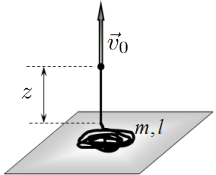
\includegraphics[width=0.3\textwidth]{Figures/Problems/Fig 1.3.png}
        \end{figure}
        \begin{enumerate}
          \item Vẽ đồ thị biểu diễn sự phụ thuộc của lực $F$ tác dụng lên xích vào độ cao $h$ của phần được nâng lên.
          \item Tính lượng nhiệt tỏa ra cho đến thời điểm sợi xích bắt đầu rời khỏi mặt bàn.
        \end{enumerate}
\end{enumerate}